
\subsection{mLSD-based optimization strategies}\label{S:mLSD}

\LSD\ stands for Lower Semi-Deviation. The \LSD\ dispersion measure can be defined as
\begin{equation}
    \LSD(r) = \left\| \left(-\br \right)^+ \right\|_2,
    \label{LSD:1}
\end{equation}
where $\br = r - \mE[r]$ is the detrended rate of return and $\|\cdot\|_2 = (\mE[|\cdot|^2])^{1/2}$ is the $L^2$-norm.

Unlike \MAD, \LSD\ is a genuine downside dispersion measure.
The \LSD-based portfolio optimization strategies were studied mainly through its
cousin, the semi-variance dispersion measure, the square of \LSD, introduced in 1959 by Markowitz \cite{Markowitz2}.
Note that semi-variance is not a genuine dispersion measure. It violates the
positive homogeneity axiom.
Nevertheless, the \LSD\ and the semi-variance optimal portfolios are the same.\footnote{Similar remarks with those made in
Sec.~\ref{CentralM} about variance and standard deviation based portfolio optimization strategies hold here.}

Like \MAD, \LSD\ can be extended to m-level \LSD. The \mLSD\ dispersion measure
is the m-level second moment downside dispersion measure from Eq.~(\ref{hmdd5}), \ie,
\begin{equation}
    \mLSD(r) = \sum_{l=1}^L \cK_l \times \delta^{(2)}_l(r),
    \label{LSD0}
\end{equation}
where $\{\cK_l\}_{l=1,\cdots,L}$ is a positive non-increasing set of coefficients normalized to unit and
$\delta^{(2)}_l$ is the $l$-th level delta-risk of second rank,
recursively defined as
\begin{align}
    \delta^{(2)}_1(r) &= \left\| \left(-\br \right)^+ \right\|_2, \label{LSD02} \\
    \cdots & \noindent \\
    \delta^{(2)}_L(r) &= \left\| \left(-\br - \sum_{j=1}^{L-1} \delta^{(2)}_j \right)^+ \right\|_2. \label{LSD01}
\end{align}


\BackToContents


\subsubsection{mLSD dispersion measure}
The numerical computation of \mLSD\ from Eq.~(\ref{LSD0}) is straightforward.
Let $L$ by the highest level involved in the expression of \mLSD. Then,
the set of $\{\delta^{(2)}_l\}_{l=1,\cdots,L}$ are evaluated recursively as follows
\begin{equation}
    \delta^{(2)}_l = \left(\frac{1}{N}\sum_{i=1}^N \left[\left( -\br_i -\sum_{j=1}^{l-1} \delta^{(2)}_j \right)^+\right]^2 \right)^{1/2}.
    \label{LSD1}
\end{equation}
The \mLSD\ is given by the sum from Eq.~(\ref{LSD0}).

\BackToContents

\subsubsection{mLSD optimal portfolio}
This optimization is described by Eqs.\ (\ref{gg1}) from Sec.~\ref{strategies} point~\ref{OptRisk},
where $\rho$ is given by \mLSD\ from Eq.~(\ref{LSD0}).
It is the following SOCP problem.

\bigskip
\noindent Minimize over $\{ \{w_k\}_{k=1,\cdots,M}, \{ \eta_l, \{ s_{li} \}_{i=1,\cdots,N} \}_{l=1,\cdots,L} \}$
\begin{subequations}\label{LSD2}
\begin{align}
    & g = \sum_{l=1}^L \cK_l \eta_l, \label{LSD2a} \\
    \st & \left( \frac{1}{N} \sum_{i=1}^N s_{li}^2 \right)^{1/2} \leq \eta_l, \label{LSD2b} \\
        & s_{li} + \sum_{k=1}^M w_k\br_{ki} + \sum_{j=1}^{l-1}\eta_j \geq 0, \label{LSD2c} \\
        & \sum_{k=1}^M w_k \mu_k \geq \mu, \label{LSD2d} \\
        & \sum_{k=1}^M w_k = 1, \label{LSD2e} \\
        & s_{li} \geq 0, \label{LSD2f} \\
        & \eta_l \geq 0, \label{LSD2h} \\
        & w_k \geq 0, \label{LSD2g}
\end{align}
\end{subequations}

\noindent where $\mu$ in Eq.~(\ref{LSD2d}) is the targeted portfolio expected rate of return while $\{\mu_k\}_{i=1,\cdots,M}$
are the portfolio components expected rate of returns.
Then, we have
\begin{subequations}\label{LSD3}
\begin{align}
    \RR &= \sum_{k=1}^m w_k^* \mu_k, \label{LSD3a} \\
    \mLSD &= g^*, \label{LSD3b} \\
    \delta^{(2)}_l & = \eta_l^*, \label{LSD3c}
\end{align}
\end{subequations}

\noindent where $^*$ denotes the solution of SOCP problem.
In addition to the portfolio weights $\{w_k^*\}_{k=1,\cdots,M}$ and optimal portfolio expected rate of return $\RR$,
the SOCP solution provides information about the portfolio \mLSD\ and its delta-risk
components.


\bigskip
\noindent Here is an example, using the \azapy\ package, of how to compute the \mLSD\ optimal portfolio.
The \mLSD\ time horizon was set to one quarter and the calibration is performed using the prior 3.25 years of
close-adjusted historical prices (default settings).
For more details see the package documentation at \azapydoc.

\lstinputlisting[language=Python]{../PyScripts/LSD_RiskOptim.py}

\BackToContents

\subsubsection{Minimum mLSD portfolio}
Following the results from Sec.~\ref{strategies} point~\ref{MinRisk}, the
algorithm to compute the optimal portfolio with minimum \mLSD\ is given by Eqs.~(\ref{LSD2}) where
$\mu$ from r.h.s. of Eq.~(\ref{LSD2d}) is set to a value equal to the smallest expected rate of
return among the portfolio components, \ie\ $\mu=\min_k\{\mu_k\}$.

\bigskip
\noindent Here is an example, using the \azapy\ package, of how to compute the minimum \mLSD\ portfolio.
The \mLSD\ time horizon was set to one quarter and the calibration is performed using the prior 3.25 years of
close-adjusted historical prices (default settings).
For more details see the package documentation at \azapydoc.

\lstinputlisting[language=Python]{../PyScripts/LSD_MinRisk.py}

\BackToContents

\subsubsection{mLSD optimal portfolio for targeted risk value}
This optimization is given by Eqs.~(\ref{gg2}) from Sec.~\ref{strategies} point~\ref{TargetRisk}, where $\rho$ is
given by $\mLSD$ from Eq.~(\ref{LSD0}).
It is the following SOCP problem.

\bigskip
\noindent Maximize over $\{ \{w_k\}_{k=1,\cdots,M}, \{ \eta_l, \{ s_{li} \}_{i=1,\cdots,N} \}_{l=1,\cdots,L} \}$
\begin{subequations}\label{LSD4}
\begin{align}
    & g = \sum_{k=1}^M w_k \mu_k, \label{LSD4a} \\
    \st & \left( \frac{1}{N} \sum_{i=1}^N s_{li}^2 \right)^{1/2} \leq \eta_l, \label{LSD4b} \\
        & s_{li} + \sum_{k=1}^M w_k\br_{ki} + \sum_{j=1}^{l-1}\eta_j \geq 0, \label{LSD4c} \\
        & \sum_{l=1}^L \cK_l \eta_l = \mLSD_0, \label{LSD4d} \\
        & \sum_{k=1}^M w_k = 1, \label{LSS4e} \\
        & s_{li} \geq 0, \label{LSD4f} \\
        & \eta_l \geq 0, \label{LSD4h} \\
        & w_k \geq 0, \label{LSD4g}
\end{align}
\end{subequations}

\noindent where $\mLSD_0$ in Eq.~(\ref{LSD4d}) is the portfolio targeted \mLSD\ dispersion value.
Then, we have
\begin{subequations}\label{LSD5}
\begin{align}
    \RR &= g^*, \label{LSD5a} \\
    \delta^{(2)}_l & = \eta_l^*, \label{LSD5b}
\end{align}
\end{subequations}

\noindent where $^*$ denotes the solution of SCOP problem.
In addition to the optimal portfolio weights $\{w_k^*\}_{k=1,\cdots,M}$ and expected rate of return $\RR$,
the SOCP solution provides information about the $\delta^{(2)}_l$ components of $\mLSD_0$,
although, this information is likely to be known at the outset.

\bigskip
\noindent Here is an example, using the \azapy\ package, of how to compute the optimal portfolio
with the same \mLSD\ as the equal weighted portfolio.
The \mLSD\ time horizon was set to one quarter and the calibration is performed using the prior 3.25 years of
close-adjusted historical prices (default settings).
For more details see the package documentation at \azapydoc.

\lstinputlisting[language=Python]{../PyScripts/LSD_InvNrisk.py}

\BackToContents

\subsubsection{mLSD optimal portfolio for fixed risk-aversion factor}
This optimization is described by Eqs.~(\ref{gg3}) from Sec.~\ref{strategies} point~\ref{RiskAverse},
where $\rho$ is given by \mLSD\ from Eq.~(\ref{LSD0}).
It is the following SOCP problem.

\bigskip
\noindent Maximize over $\{ \{w_k\}_{k=1,\cdots,M}, \{ \eta_l, \{ s_{li} \}_{i=1,\cdots,N} \}_{l=1,\cdots,L} \}$
\begin{subequations}\label{LSD6}
\begin{align}
    & g = \sum_{k=1}^M w_k\mu_k - \lambda \sum_{l=1}^L \cK_l \eta_l, \label{LSD6a} \\
    \st & \left( \frac{1}{N} \sum_{i=1}^N s_{li}^2 \right)^{1/2} \leq \eta_l, \label{LSD6b} \\
        & s_{li} + \sum_{k=1}^M w_k\br_{ki} + \sum_{j=1}^{l-1}\eta_j \geq 0, \label{LSD6c} \\
        &\sum_{k=1}^M w_k = 1, \label{LSD6d} \\
        & s_{li} \geq 0, \label{LSD6e} \\
        & \eta_l \geq 0, \label{LSD6g} \\
        & w_k \geq 0, \label{LSD6f}
\end{align}
\end{subequations}

\noindent where $\lambda$ from Eqs.~(\ref{LSD6a}) is the risk-aversion factor.
Then, we have
\begin{subequations}\label{LSD7}
\begin{align}
    \RR &= \sum_{k=1}^M w_k^* \mu_k, \label{LSD7a} \\
    \mLSD &= \frac{\RR - g^*}{\lambda}, \label{LSD7b} \\
    \delta^{(2)}_l &= \eta_l^*, \label{LSD7c}
\end{align}
\end{subequations}

\noindent where $^*$ denotes the solution of the SOCP problem.
In addition to the optimal portfolio weights $\{w_k^*\}_{k=1,\cdots,M}$ and expected rate of return $\RR$,
the SOCP solution provides information about the portfolio \mLSD\ and its delta-risk components.

\bigskip
\noindent Here is an example, using the \azapy\ package, of how to compute the optimal portfolio
for a given value of the risk-aversion factor.
The \mLSD\ time horizon was set to one quarter and the calibration is performed using the prior 3.25 years of
close-adjusted historical prices (default settings).
For more details see the package documentation at \azapydoc.

\lstinputlisting[language=Python]{../PyScripts/LSD_Averse.py}

\BackToContents

\subsubsection{mLSD-Sharpe optimal portfolio - maximization solution}
This optimization targets the maximization of \mLSD-Sharpe ratio. It is based on the
Eqs.~(\ref{gg4}) from Sec.~\ref{strategies} point~\ref{MaxSharpe},
where $\rho$ is given by \mLSD\ from Eq.~(\ref{LSD0}).
The optimization can be formulated as an SOCP problem if Eq.~(\ref{gg4b}) can be expressed as a second order cone constraint.
This can be achieved by
introducing the variable transformations $\bw_k = t w_k$, $\bs_{li} = t s_{li}$ and $\bbeta_l = t \eta_l$.
Then, the SOCP problem can be written as follows.

\bigskip
\noindent Maximize over $\{ \{\bw_k\}_{k=1,\cdots,M}, \{ \bbeta_l, \{ \bs_{li} \}_{i=1,\cdots,N} \}_{l=1,\cdots,L}, t \}$
\begin{subequations}\label{LSD8}
\begin{align}
    &  g = \sum_{k=1}^M \bw_k \mu_k - \mu_0 t, \label{LSD8a} \\
    \st & \left( \frac{1}{N} \sum_{i=1}^N \bs_{li}^2 \right)^{1/2} \leq \bbeta_l, \label{LSD8b} \\
        & \bs_{li} + \sum_{k=1}^M \bw_k\br_{ki} + \sum_{j=1}^{l-1}\bbeta_j \geq 0, \label{LSD8c} \\
        & \sum_{l=1}^L \cK_l \bbeta_l = 1, \label{LSD8d} \\
        & \sum_{k=1}^M \bw_k - t = 0, \label{LSD8e} \\
        & t \geq 0, \label{LSD8h} \\
        & \bs_{li} \geq 0, \label{LSD8f} \\
        & \bbeta_l \geq 0, \label{LSD8i} \\
        & \bw_k \geq 0, \label{LSD8g}
\end{align}
\end{subequations}

\noindent where $\mu_0$ from Eq.~(\ref{LSD8a}) is the risk-free rate accessible to the investor.
Then, we have
\begin{subequations}\label{LSD9}
\begin{align}
    w_k &= \frac{\bw_k^*}{t^*}, \label{LLSD9a} \\
    \RR &= \frac{g^*}{t^*} + \mu_0, \label{LSD9b} \\
    \Sharpe &= g^*, \label{LSD9c} \\
    \mLSD & = \frac{1}{t^*}, \label{LSD9d} \\
    \delta^{(2)}_l &= \frac{\bbeta_l^*}{t^*}, \label{LLSD9e}
\end{align}
\end{subequations}

\noindent where $^*$ denotes the solution of SOCP problem.
In addition to the optimal portfolio weights $\{w_k\}_{k=1,\cdots,M}$, expected rate of return $\RR$ and
\mLSD-Sharpe ratio $\Sharpe$,
the SOCP solution provides information about the portfolio \mLSD\ and its delta-risk components.

\bigskip
\noindent Here is an example, using the \azapy\ package, of how to compute the \mLSD-Sharpe optimal portfolio using the maximization
of \mLSD-Sharpe ratio.
The \mLSD\ time horizon was set to one quarter and the calibration is performed using the prior 3.25 years of
close-adjusted historical prices (default settings).
For more details see the package documentation at \azapydoc.

\lstinputlisting[language=Python]{../PyScripts/LSD_Sharpe.py}

\BackToContents


\subsubsection{mLSD-Sharpe optimal portfolio - minimization solution}
This optimization targets the minimization of the inverse of \mLSD-Sharpe ratio.
It is  described by Eqs.~(\ref{gg8}) from Sec.~\ref{strategies} point~\ref{MinSharpe}, where
$\rho$ is given by \mLSD\ from Eq.~(\ref{LSD0}).
The optimization can be formulated as an SOCP problem if  Eq.~(\ref{gg8a}) can be expressed as a second order cone constraint.
This can be achieved by
introducing the variable transformations
$\bw_k = t w_k$, $\bs_{li} = t s_{li}$ and $\bbeta_l = t \eta_l$.
Then, the SOCP problem can be written as follows.

\bigskip
\noindent Minimize over $\{ \{\bw_k\}_{k=1,\cdots,M}, \{ \bbeta_l, \{ \bs_{li} \}_{i=1,\cdots,N} \}_{l=1,\cdots,L}, t \}$
\begin{subequations}\label{LSD10}
\begin{align}
    & g = \sum_{l=1}^L \cK_l \bbeta_l, \label{LSD10a} \\
    \st & \left( \frac{1}{N} \sum_{i=1}^N \bs_{li}^2 \right)^{1/2} \leq \bbeta_l, \label{LSD10b} \\
        & \bs_{li} + \sum_{k=1}^M \bw_k\br_{ki} + \sum_{j=1}^{l-1}\bbeta_j \geq 0, \label{LSD10c} \\
        & \sum_{k=1}^M \bw_k \mu_k -\mu_0 t = 1, \label{LSD10d} \\
        & \sum_{k=1}^M \bw_k - t = 0, \label{LSD10e} \\
        & t \geq 0, \label{LSD10f} \\
        & \bs_{li} \geq 0, \label{LSD10g} \\
        & \bbeta_l \geq 0, \label{LSD11h} \\
        & \bw_k \geq 0, \label{LSD10i}
\end{align}
\end{subequations}

\noindent where $\mu_0$ from Eq.~(\ref{LSD10d}) is the risk-free rate accessible to the investor.
Then, we have
\begin{subequations}\label{LSD11}
\begin{align}
    w_k &= \frac{\bw_k^*}{t^*} , \label{LSD11a} \\
    \RR &= \frac{1}{t^*} + \mu_0, \label{LSD11b} \\
    \Sharpe &= \frac{1}{t^*}, \label{LSD11c} \\
    \mLSD &= \frac{g^*}{t^*}, \label{LSD11d} \\
    \delta^{(2)}_l &= \frac{\bbeta_l^*}{t^*}, \label{LSD11e}
\end{align}
\end{subequations}

\noindent where $^*$ denotes the solution of SOCP problem.
In addition to the optimal portfolio weights $\{w_k\}_{k=1,\cdots,M}$, expected rate of return $\RR$ and
\mLSD-Sharpe ratio $\Sharpe$,
the SOCP solution provides information about the portfolio \mLSD\ and its delta-risk components.

\bigskip
\noindent Here is an example, using the \azapy\ package, of how to compute the \mLSD-Sharpe optimal portfolio using the minimization
of the inverse of \mLSD-Sharpe ratio.
The \mLSD\ time horizon was set to one quarter and the calibration is performed using the prior 3.25 years of
close-adjusted historical prices (default settings).
For more details see the package documentation at \azapydoc.

\lstinputlisting[language=Python]{../PyScripts/LSD_InvSharpe.py}

\BackToContents

\subsubsection{mLSD frontiers}

Here is an example of how to compute the \mLSD\ frontiers using the \azapy\
package. The \mLSD\ time horizon was set to one quarter and the calibration is performed using the prior 3.25 years of
close-adjusted historical prices (default settings).
For more details see the package documentation at \azapydoc.

The script will produce the plots in Figs. \ref{LSD_fig1a} and \ref{LSD_fig1b}
for historical data collected up to 2021-07-27.

\lstinputlisting[language=Python]{../PyScripts/LSD_frontiers.py}

\begin{figure}[H]
\centering
\begin{subfigure}{.5\textwidth}
  \centering
  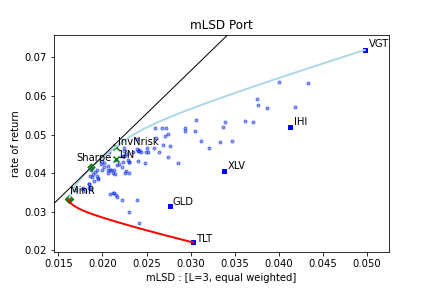
\includegraphics[width=.95\linewidth]{../figs/mLSDFrontier1.png}
  \caption{Rate of return vs. \mLSD}
  \label{LSD_fig1a}
\end{subfigure}%
\begin{subfigure}{.5\textwidth}
  \centering
  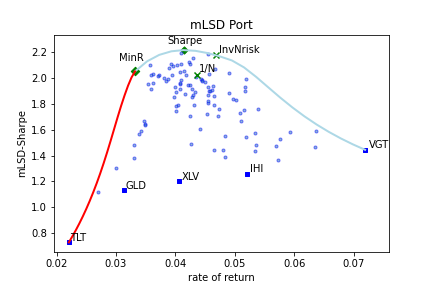
\includegraphics[width=.95\linewidth]{../figs/mLSDFrontier2.png}
  \caption{\mLSD-Sharpe vs. rate of return}
  \label{LSD_fig1b}
\end{subfigure}
\caption{\mLSD : [$L=3$, equal weighted], frontiers.}
\label{LSD_fig1}
\end{figure}

\BackToContents


\subsubsection{Backtesting mLSD-Sharpe optimal portfolio}

Here is an example, using \azapy\ package, of computing a portfolio backtesting.
For this example, we have chosen a portfolio quarterly rebalanced according
to the maximization of \mLSD-Sharpe ratio. At each rebalancing date,
the portfolio weights
are calibrated based on 3.25 years of prior historical market data.

Other rebalancing strategies can be considered
by changing the value of {\it rtype} parameter in the call of {\it set\_model} function below.
For more details see the package documentation at \azapydoc.

\lstinputlisting[language=Python]{../PyScripts/LSD_Port.py}

\begin{figure}[H]
    \centering
    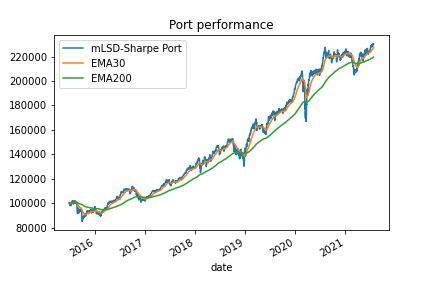
\includegraphics[width=.95\linewidth]{../figs/Port_mLSD_Sharpe.png}
    \caption{Backtesting of quarterly rebalanced \mLSD-Sharpe optimal portfolio,
    \mLSD\ : [$L=3$, equal weighted].}
    \label{LSD_Port_fig}
\end{figure}

\BackToContents
